\documentclass[../document.tex]{subfiles}

\begin{document}


\section{Architecture}
\subsection{Introduction}
This chapter gives an overview of the architectural structure of the system, including quality attributes, and architectural styles, constraints, tactics and views. This is the architecture we plan on following, and any changes made during the implementation will be documented.

\subsection{Quality attributes}
\subsubsection{Functionality}
The system consists of multiple sensor devices, a central hub, and one or more client devices. The sensors gather data from an environment, such as temperature, light level, or sound, and move it to a central hub. A client device collects sensor data from the central hub, and visualizes the data in a grand manner.

\subsubsection{Performance}
The system is a real time system, and changes in the environment is registered at the client within five seconds. Also, all transfer links in the system has sufficient throughput to avoid delay or lost packages.

\subsubsection{Scalability}
The system is scaleable to a large degree, and supports adding many sensor devices.

\subsubsection{Modifiability of components}
The software is easy to alter or configure, to ease system modifications such as moving or removing components, or relocating the system.

\subsubsection{Portability of components}
The program code for both the central hub and the sensors is portable, making the system hardware replaceable. This is to ensure that a customer is not tied to any specific supplier. The data should be stored in a database.

\subsection{Architectural styles}
\subsubsection{Representational state transfer (REST)}
We plan to make a system with a RESTful similarity between the collector and the central hub. The architectural style REST focus on how components, connectors and data elements works together within a distributed hypermedia system. REST will accomplish that by having a set of architectural constraints that applies to all modules and their relations. The individual module is not concerned in REST architecture, meaning that the implementation is not that important. The architectural constraints applied by REST can be found under architectural constraints. REST is used as a description of the wanted web architecture. We use it to find and identify problems in our system architecture and make sure our system should follow the constraint we find to be more important. As in any software architecture the components, the connectors and the data elements are used to find what architectural properties are most needed in the system. Our components, connectors and data elements are as listed:

\begin{table}[H]
	\caption{Identified REST elements}
	\begin{tabularx}{\textwidth}{|X|X|}
		\hline
		\textbf{Components}		& The sensors, the central hub, the database and the UI.  \\ \hline
		\textbf{Connectors}		& The collector who ask on-demand for the data the central hub receives from the sensors.  \\ \hline
		\textbf{Data elements}	& The information sent from the sensors through every component in the system until it reaches  the visualization.  \\ \hline
	\end{tabularx}
\end{table}

We are using the REST style as guidelines, and therefore it may be some inconsistencies between our system and a RESTful system. 

\subsection{Architectural constraints}
REST has some formal constraints we have to follow. If the system does not follow these constraints the system does not have RESTful architecture. They are all written with an interest to our system and architecture.

\subsubsection{Client-Server}
The central hub will act as a server, and a data collector as the client. All the data is stored in a database that may be run on either the central hub, or externally. The data collector will only ask for data from the central hub and will not be storing any data, it will just push the data into the database. Having the data collector not worrying about the storage improves the portability of the code for the data collector. The central hub will not be worrying about the UI or any kind of user interference or status. This makes the central hub more scalable and it can be developed or changed without the data collector knowing if the interface between them are altered or not. 

\subsubsection{Stateless}
When the data collector asks for a data update from the central hub, all the information needed for the central hub to do what is requested is in the request sent from the data collector. All the states of the data collector is only for the data collector to see. The central hub should not be concerned with which state the data collector is in. The data collector have 4 different states which are state 1: send request, state 2: pull data, state 3: manipulate data and state 4: send data.

\subsubsection{Cacheable}
The data collectors in our system will be able to cache the data it receives from the central hub before it pushes the data into the database. Data collectors can therefore lookup data in its cache if it needs the data once more without sending a new request to the central hub. This will improve the scalability and the performance. 

\subsubsection{Layered system}
Our system might not be layered, so the data collector will most likely know for certain that it is connected to the central hub. This is not usually how the REST architecture acts, however we are only having a RESTful system as a framework. 

\subsubsection{Code on demand (optional)}
This is the only architectural constraint that is optional with the REST architecture, and we have decided it is not going to be a concern with our system. However, the formal description of this constraint is: Code on demand allows clients to improve its flexibility by temporarily letting the servers extend or customize the functionality of a client. This is done by transferring executable code.

\subsubsection{Uniform interface}
This constraint is used to make the architecture simpler and helps every individual part of the system to evolve independently. The uniform interface is split into four different guidelines.

\paragraph{Identification of resources} \ \\
The resources in a REST architecture is identified in the requests and are separate from the representations that the client receives. 

\paragraph{Manipulation of resources through these representations} \ \\
The client should be able to modify the representation of a resource it receives. As an example the client could be able to calculate maximum, minimum and average of data from each sensor. 

\paragraph{Self-descriptive messages} \ \\
All the client requests and server responses are messages, and in a RESTful application these messages are expected to be self-descriptive. This means that each message should contain all the information needed to process this message. Moreover, the interaction between requests is stateless, responses explicitly indicate cacheability and standard methods and media types are used to indicate semantics and exchange information. Each message can have a body and metadata.

\paragraph{Hypermedia as the engine of application state (A.K.A. HATEOAS)}
The principle that hypermedia is the engine of application state means that a REST client does not need to have any understanding of how to interact with any application or server beyond a generic understanding of hypermedia. In other words, except for simple entry points in the application, a client does not make any state transitions without hypermedia dynamically provided by the server. 

\subsection{Architectural tactics}
\subsubsection{Performance}
To achieve the performance attribute we will let the client be able to cache the data it receives from the server before it pushes it into the database. In this way the client can lookup data in its cache without sending a new request to the server.

\subsubsection{Scalability}
As mentioned earlier, the server will not be worrying about any kind of user interference, status or UI and, the client will be able to lookup data in its cache if it needs it once more. This makes the server more scalable.

\subsubsection{Modifiability of components}
To ensure that the system can be easily changed we will use the abstract common services tactic. To abstract common services is when services that provide similar services is implemented once in a general module instead of many times in slightly different but more specific modules. When the common services are abstracted, modifications to them will need to be made to only one module instead of in each module where the services are used. This tactic also supports the prevention of ripple effects because the modifications to the modules that uses these services will not impact other modules.

\subsubsection{Portability of components}
To improve the portability we will only let the client ask for data from the server, and not store any data. In this way, the client does not need to worry about the storage and this improves the portability of the code for the client.

\subsection{Stakeholders and concerns}
\begin{table}[H]
	\caption{Stakeholders}
	\begin{tabularx}{\textwidth}{|X|X|}
		\hline
		\textbf{Stakeholders}	& \textbf{Descriptions} \\ \hline
		End user				& The end user is the future clients who will use our system.  \\ \hline
		Developers				& The developer are us in group 10 and our job is to develop the product and document the project.  \\ \hline
		Customer				& The customer is Stig Lau representing Altran AS. He will specify the product to be developed.  \\ \hline
		Advisor					& The advisor is Mohsen Anvaari. His job is to act as a project management.  \\ \hline
		Course staff			& The course staff for subject TDT4290 will provide information and prestudy for the course.  \\ \hline
		Hardware suppliers		& The hardware suppliers are the makers for the components used in this project.  \\ \hline
	\end{tabularx}
\end{table}

\paragraph{End user:} The end user is the future clients who will use the system. They can watch the visualization form the data gathered from a room on a web page or similar. 

\paragraph{Developers:} The developers in this project is us in group 10. Our job is to plan, implement and test the wanted product. We will start with planning, and then write requirement and architecture documents. When the documentation is done, we will implement the system in Scrum-style sprints. During implementation, we will follow our test plan until the customer is satisfied and the product is finished. We might add test results, changes and issues we had along the way and finish the report and deliver it to the customer.

\paragraph{Customer:} The customer is Stig Lau representing Altran AS. He specify the product to be developed, and will meet with the developers to agree on details and clear out discrepancies around the product implementation. He has the final word when it comes to what functions the system should and should not have. He is also the developers guide on how the sensors and central hub supplied by Altran works, and what can be done with them.

\paragraph{Adviser:} The groups advisor is Mohsen Anvaari. He will give feedback and guide the developers on all areas. This will be done by giving feedback and help us create a good documentation, and help us with any issues we might have that does not concern the client.

\paragraph{Course staff:} The course staff for subject TDT4290 will be a part of the prestudy as they hold lectures needed for the course, and guidelines and tips for the project. 

\paragraph{Hardware suppliers:} The hardware suppliers in this project are the developers of the components used in this project. They are delivering all of the parts needed for the sensors and the central hub.

\subsection{Architectural views}
\subsubsection{Introduction}
In this section we will show the different views of our architecture. We will follow the structure of the 4+1 View Model of Software Architecture. We chose this view model because it allows us to handle the functional and nonfunctional requirements separately, and also address the different concerns of the various stakeholders separately. 

\subsubsection{Logical view}		
The logical view is primarily concerned with the functional requirements. In other words, it is concerned with what the system should provide in terms of services to its end-users. Our logic view uses a class diagram to demonstrate the logical interaction between the client, the database, the gui, the gatherer, the server, and the sensors. The class diagram was to big at the first draft, so to make it fit the document we cut down on the methods and fields that were unnecessary such as getters and setters, and when every data type (temperarture, lighting, humidity and pressure) have methods and/or fields each we wrote "(Data type)" to represent the data types, that way we don't repeat ourself four times. 

\begin{figure}[H]
	\centering
	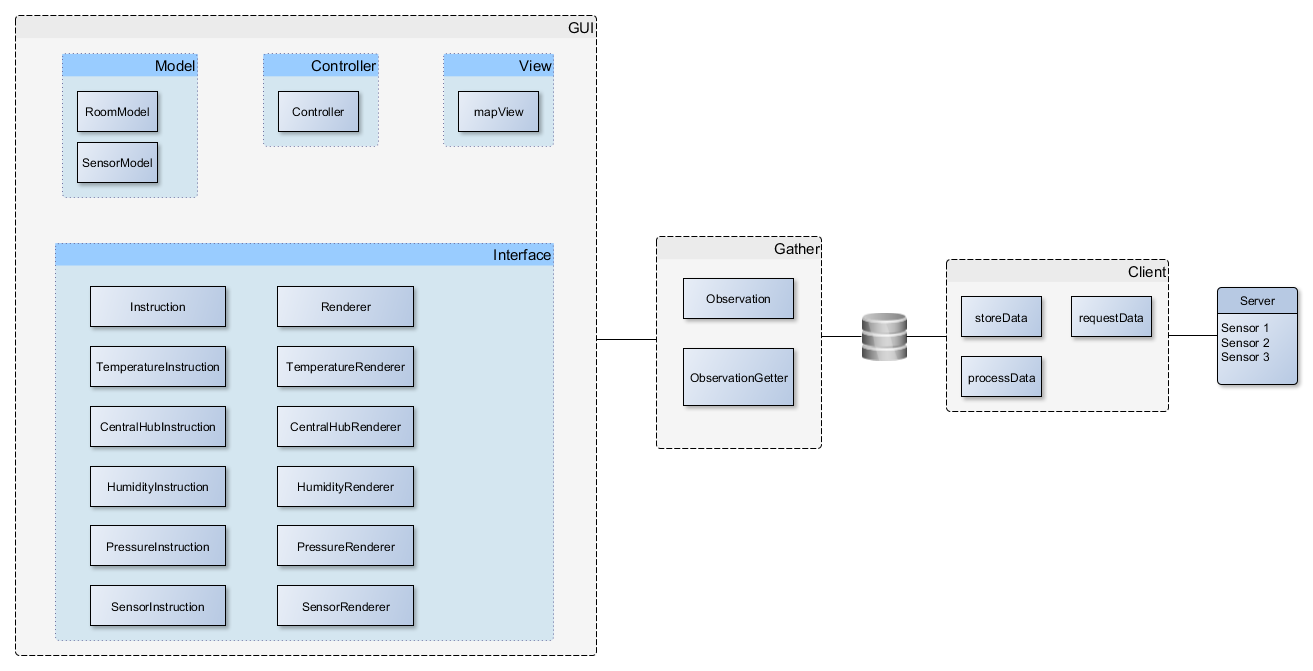
\includegraphics[width=\textwidth]{Architecture/LogicalView.png}
	\caption{Logical View}
\end{figure}

\subsubsection{Development view}
The development view, also known as the implementation view,  presents the system from a programmers perspective and is concerned with software management. Our development view shows the relationships between importing and exporting information from and to the database. It shows that the client stores the information from the sensors in the database and that the visualizer get this information from the database.

\begin{figure}[H]
	\centering
	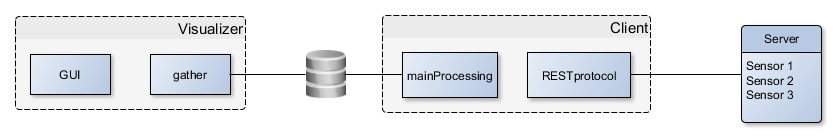
\includegraphics[width=\textwidth]{Architecture/DevelopmentView.png}
	\caption{Development View}
\end{figure}

\subsubsection{Process view}
The process view considers the dynamic aspects of the system. It explains the system processes and how they communicate, and focuses on the runtime behavior of the system. We use an activity diagram to present how the different parts in the system are connected. The parts include the checkboxes that decides which elements the user wants to see. 

\begin{figure}[H]
	\centering
	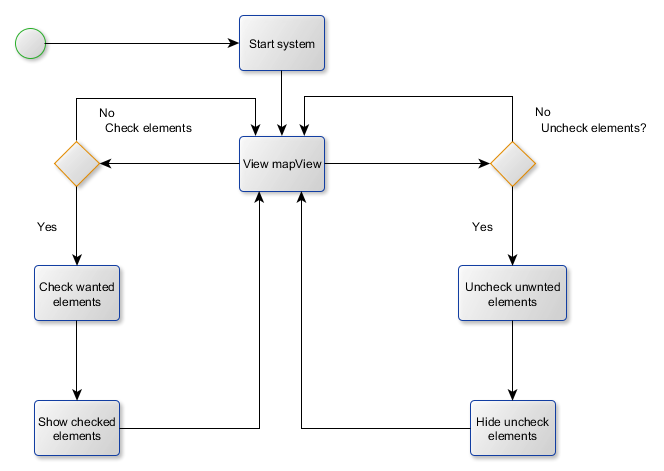
\includegraphics[width=\textwidth]{Architecture/ProcessviewNew.png}
	\caption{Process View}
\end{figure}

\subsubsection{Physical view}
The physical view, also known as the deployment view, is concerned with the topology of software components on the physical layer, as well as the physical connections between these components. In other words, it depicts the system from a system engineers point of view. The sensors are all somehow connected to the REST server, which gives information about the sensors to the database through the REST client. If the sensors for some reason are not used then the database gets random information from a data collector mock. The user interface gets information from the database.

\begin{figure}[H]
	\centering
	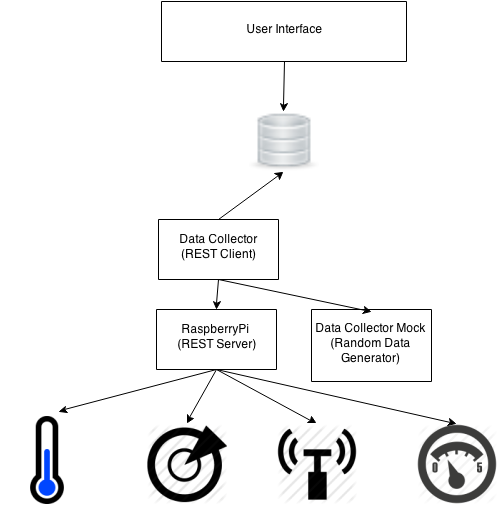
\includegraphics[width=\textwidth]{Architecture/System_Diagram.png}
	\caption{System Diagram}
\end{figure}

\subsubsection{Scenarios and use cases}
\paragraph{Scenarios} \ \\
The scenarios view, also known as the use case view, describe sequences of interactions between objects, and between processes. They are used to identify architectural elements and to illustrate and validate the architecture design. They also serve as a starting point for tests of an architecture prototype.

\begin{table}[H]
	\caption{Scenario P1}
	\begin{tabularx}{\textwidth}{|X|X|}
		\hline
		ID					& P1 \\ \hline
		Source				& System \\ \hline
		Stimulus			& The light gets turned off \\ \hline
		Environment			& Runtime \\ \hline
		Artifact			& Light sensors \\ \hline
		Response			& Update the new info, and add it to the database \\ \hline
		Response Measure	& Time \newline Should be less than 30 seconds
		\\ \hline
	\end{tabularx}
\end{table}

\begin{table}[H]
	\caption{Scenario P2}
	\begin{tabularx}{\textwidth}{|X|X|}
		\hline
		ID					& P2 \\ \hline
		Source				& System \\ \hline
		Stimulus			& The temperature gets higher \\ \hline
		Environment			& Runtime \\ \hline
		Artifact			& Temperature sensors \\ \hline
		Response			& The animation in the visualizer should start after it pulls new data from the database \\ \hline
		Response Measure	& Time\newline Should be less than 30 seconds
		\\ \hline
	\end{tabularx}
\end{table}

\paragraph{Use cases} \ \\
The use cases shows two ways a user can interact with the system. The first shows how a user can uncheck elements it does not want to see on the screen and second shows how the user can check them back if the user wants to see them again.

\begin{figure}[H]
	\centering
	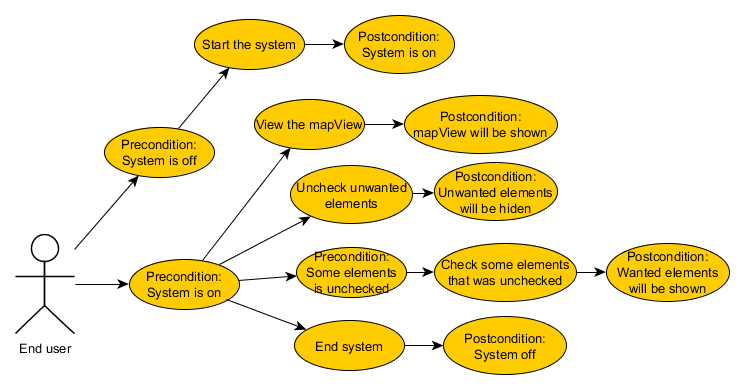
\includegraphics[width=\textwidth]{Architecture/usecaseUncheck.png}
	\caption{Use Case Uncheck}
\end{figure}

\begin{figure}[H]
	\centering
	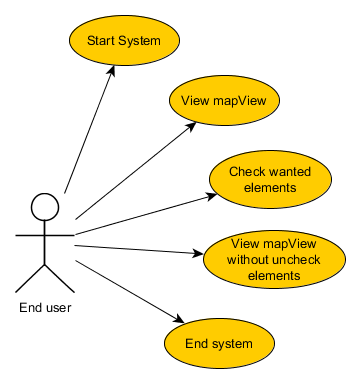
\includegraphics[width=\textwidth]{Architecture/usecaseCheck.png}
	\caption{Use Case Check}
\end{figure}

\end{document}
